% -*- program: xelatex -*-
\documentclass[11pt, compress]{beamer}
%\usepackage{listings}

\usepackage{pgfpages}

%\documentclass{article}
%\usepackage{beamerarticle}

%\documentclass[12pt, compress]{beamer} 
%\documentclass[notes=only]{beamer}

\usepackage{fontspec}

\setsansfont{PT Sans}
\setmonofont{PT Mono}

\usepackage{beamerthemesplit}
\usefonttheme[onlymath]{serif}
%\DeclareFontEncoding{T1}
\fontencoding{T1}

%\usepackage[T2A]{fontenc}
%\usepackage[utf8]{inputenc}
\usepackage[russian]{babel}
\usepackage{listings}


\usepackage{amsmath,amssymb,amsthm}
\hypersetup{unicode=true}

\usepackage{color}
\definecolor{mygred}{RGB}{150,0,0} 
\definecolor{mygreen}{RGB}{28,172,0} 
\definecolor{mylilas}{RGB}{170,55,241}
\definecolor{codecolor}{RGB}{0,120,0}
\definecolor{emphcolor}{RGB}{0,0,120}
\definecolor{gray}{RGB}{150,150,150}

\definecolor{light-gray}{gray}{0.95}
\definecolor{light-green}{rgb}{0.93, 1, 0.8}
\definecolor{light-yellow}{rgb}{1,1,0.85}
\definecolor{light-red}{rgb}{0.8, 0.3, 0.3}

\definecolor{dark-blue}{rgb}{0,0,0.6}
\definecolor{dark-red}{rgb}{0.7,0.0,0.0}
\definecolor{dark-green}{RGB}{10,150,0}

\usepackage{pifont}% http://ctan.org/pkg/pifont
\newcommand{\cmark}{\textcolor{green}{\ding{51}}}
\newcommand{\xmark}{\textcolor{red}{\ding{55}}}

\newcommand{\matcode}[1]{ \textcolor{codecolor}{\texttt{#1}}}
\usepackage{graphics,graphicx}
\usepackage{verbatim}
\usepackage{fancyvrb}
\usepackage{booktabs}
%\usepackage{media9}

\usepackage[super]{natbib}
 
\newcommand{\cleartitlepage}[1]{\begin{frame}[plain]\begin{center}\textsc{#1}\end{center}\end{frame}}

\renewcommand{\emph}[1]{\textcolor{emphcolor}{#1}}
\newcommand{\emphb}[1]{\textcolor{emphcolor}{\textbf{#1}}}


\usetheme{CambridgeUS}
\usecolortheme{lily}

\usepackage{tikz}
\usetikzlibrary{positioning} 
\tikzset{cbutton/.style={rectangle,minimum width=10mm,thick,draw=red!50!black!50,
top color=white,bottom color=red!50!black!30}}
\tikzset{mbutton/.style={rectangle,minimum width=10mm,thick,draw=black!20,
top color=white,bottom color=black!30}}


\lstset{basicstyle=\ttfamily\footnotesize,
    language=Python,    
    keepspaces=true,
    extendedchars=true,
    basicstyle={\footnotesize  \color{black}},
    breaklines=true,    
    keywordstyle=\color{blue},
    morekeywords=[2]{1}, keywordstyle=[2]{\color{codecolor}},
    identifierstyle={ \bf \color{black} },
    stringstyle=\color{mylilas},
    commentstyle=\color{mygreen},%
    showstringspaces=false,
    numbers=left,%
    numberstyle={\tiny \color{black}},
    numbersep=7pt, 
    emph=[1]{case,switch,otherwise},emphstyle=[1]\color{blue}, 
    frame=single,    
    rulecolor=\color{red},    
    backgroundcolor=\color{light-gray},
    xleftmargin=0.3cm,
    frame=l,framesep=4pt,framerule=0.5pt,
    showspaces=false,
    escapechar=|
    %lineskip=-0.3pt,
    %emph=[2]{word1,word2}, emphstyle=[2]{style},    
}

\setbeamertemplate{blocks}[rounded][shadow=false]
\setbeamertemplate{navigation symbols}{}

\makeatother
\setbeamertemplate{footline}
{
  \leavevmode%
  \hbox{%
  \begin{beamercolorbox}[wd=.3\paperwidth,ht=2.25ex,dp=1ex,center]{author in head/foot}%
    \usebeamerfont{author in head/foot}\insertshortauthor
  \end{beamercolorbox}%
  \begin{beamercolorbox}[wd=.6\paperwidth,ht=2.25ex,dp=1ex,center]{title in head/foot}%
    \usebeamerfont{title in head/foot}\insertshorttitle
  \end{beamercolorbox}%
  \begin{beamercolorbox}[wd=.1\paperwidth,ht=2.25ex,dp=1ex,center]{date in head/foot}%
    \insertframenumber{} / \inserttotalframenumber\hspace*{1ex}
    %\insertframenumber{} \hspace*{0.1ex}
  \end{beamercolorbox}}%
  \vskip0pt%
}


% define colours
% taken from pickton on Adobe Kuler:
% https://kuler.adobe.com/Some-Kind-Of-Execushares-color-theme-3837185/
 \definecolor{ExecusharesRed}{RGB}{230,37,52}
 \definecolor{ExecusharesBlack}{RGB}{43,40,40}
 \definecolor{ExecusharesBlue}{RGB}{22,190,207}
 \definecolor{ExecusharesWhite}{RGB}{255,255,243}
 \definecolor{ExecusharesGrey}{RGB}{107,110,108}

% \setbeamertemplate{itemize item}{
%  \tikz{
%    \draw[fill=emphcolor,draw=none] (0, 0) rectangle(0.1, 0.1);
%    \draw[fill=emphcolor,draw=none] (0.1, 0.1) rectangle(0.2, 0.2);
%    \draw[fill=emphcolor,draw=none] (0, 0.2) rectangle(0.1, 0.3);
%  }
% }

\AtBeginSection[]{
  \begin{frame}[plain]
  %\vfill  
  \begin{tikzpicture}
  \useasboundingbox (0,0) rectangle(\the\paperwidth,\the\paperheight);  
  \fill[color=mygred]   (-1cm, 3.9cm) rectangle(\the\paperwidth, 5.9cm);
  %\usebeamerfont{title}\insertsectionhead\par%
  %\node[text width=\the\paperwidth,align=center] at (current page.center) {\color{ExecusharesWhite}\Large\textbf{\insertsectionhead}};  
  \node[text width=\the\paperwidth,align=center] at (6cm,4.9cm) {\color{ExecusharesWhite}\Large\textbf{\insertsectionhead}};  
  \end{tikzpicture}
  \end{frame}
}

\setbeamertemplate{headline}{}
\setbeamertemplate{footline}{}

\makeatother
\setbeamertemplate{footline}
{
  \leavevmode%
  \hbox{%  
  \begin{beamercolorbox}[wd=.3\paperwidth,ht=2.25ex,dp=1ex,center]{author in head/foot}%
    \usebeamerfont{author in head/foot}\insertshortauthor
  \end{beamercolorbox}%  
  \begin{beamercolorbox}[wd=.6\paperwidth,ht=2.25ex,dp=1ex,center]{title in head/foot}%
    \usebeamerfont{title in head/foot}\insertshorttitle
  \end{beamercolorbox}%
  \begin{beamercolorbox}[wd=.1\paperwidth,ht=2.25ex,dp=1ex,center]{date in head/foot}%
    \insertframenumber{} \hspace*{1ex}
  \end{beamercolorbox}}%
  \vskip0pt%
}

\setbeamercolor{frametitle}{fg=dark-red,bg=gray!10}
\setbeamerfont{title}{series=\bfseries,parent=structure}
\setbeamerfont{frametitle}{series=\bfseries,parent=structure}

%\usepackage{media9}

\definecolor{dark-blue}{rgb}{0,0,0.6}
\definecolor{dark-red}{RGB}{204,0,0}
\definecolor{dark-green}{RGB}{28,172,0}

\lstset{language=Matlab,    
    keepspaces=true,
    extendedchars=true,
    basicstyle={\footnotesize  \color{black}},
    breaklines=true,
    morekeywords={matlab2tikz}, 
    keywordstyle=\color{blue},
    morekeywords=[2]{1}, keywordstyle=[2]{\color{codecolor}},
    identifierstyle={ \bf \color{black} },
    stringstyle=\color{mylilas},
    commentstyle=\color{mygreen},%
    showstringspaces=false,
    numbers=left,%
    numberstyle={\tiny \color{black}},
    numbersep=7pt,  
    emph=[1]{case,switch,otherwise},emphstyle=[1]\color{blue}, 
    frame=single,    
    %lineskip=-1.0pt,
    %emph=[2]{word1,word2}, emphstyle=[2]{style},    
}

\title{Численные методы}
\subtitle{Основы MATLAB}
\author[Кафедра теоретической механики]{Юдинцев В. В.}
\small
\institute{Кафедра теоретической механики}


\begin{document}

{
\usebackgroundtemplate{
\includegraphics[width=\paperwidth,height=\paperheight]{back.png}}
\begin{frame}[plain] 
\maketitle
\end{frame}
}

\frame{
\frametitle{Содержание}
\tableofcontents
}

\section{Интерполирование табличных данных}
%
%
\frame{
\frametitle{Полиномиальная интерполяция}
\begin{itemize}
 \item Известны значения некоторой функции $y(x)$ в точках $x_0, x_1, x_2, \ldots, x_n$:
$$
  y_0, y_1, y_2, \ldots, y_n.
$$  
 \item Необходимо построить интерполирующий многочлен $L_{n}(x)$, совпадающий с значениями табличной функции в точках $x_0, x_1, x_2, \ldots, x_n$ и приближающий функцию $y(x)$ на интервале $[x_0,x_n]$.
\end{itemize}
}

\subsection*{Полиномы}

\begin{frame}[fragile]
\frametitle{Полиномы}
Для определения коэффициентов интерполяционного полинома, проходящего через заданные точки с координатами $x_1, f(x_1)$, $x_2, f(x_2)$, ... $x_n, f(x_n)$ используется функция \matcode{polyfit}:
\begin{lstlisting}
>> x = [ 1  2  3  4 ];
>> y = [ 0  0.6931  1.0986  1.3863 ];
>> p = polyfit(x, y, 3)
\end{lstlisting}
Аргументы:
\begin{itemize}
\item Список значений $x_0, x_1, x_2, \ldots, x_n$
\item Список значений $y_0, y_1, y_2, \ldots, y_n$
\item Степень полинома
\end{itemize}
\end{frame}

\begin{frame}[fragile]
    \frametitle{Полиномы}    
    \begin{lstlisting}
    >> x = [ 1  2  3  4 ];
    >> y = [ 0  0.6931  1.0986  1.3863 ];
    >> p = polyfit(x, y, 3)
    
    p =
    
        0.0283   -0.3137    1.4362   -1.1507
    \end{lstlisting}
    Результат -- коэффициенты полинома
    $$
        0.0283 x^3 - 0.3137 x^2 + 1.4362 x - 1.1507
    $$
\end{frame}
    

\frame[containsverbatim]
{
\frametitle{Построение графика}
\begin{lstlisting}[firstnumber=last]
>> fplot(@(xa) polyval(p,xa),[x(1), x(end)]);
>> print('-dpng', '-r600', 'function.png');
\end{lstlisting}      
\begin{center}
 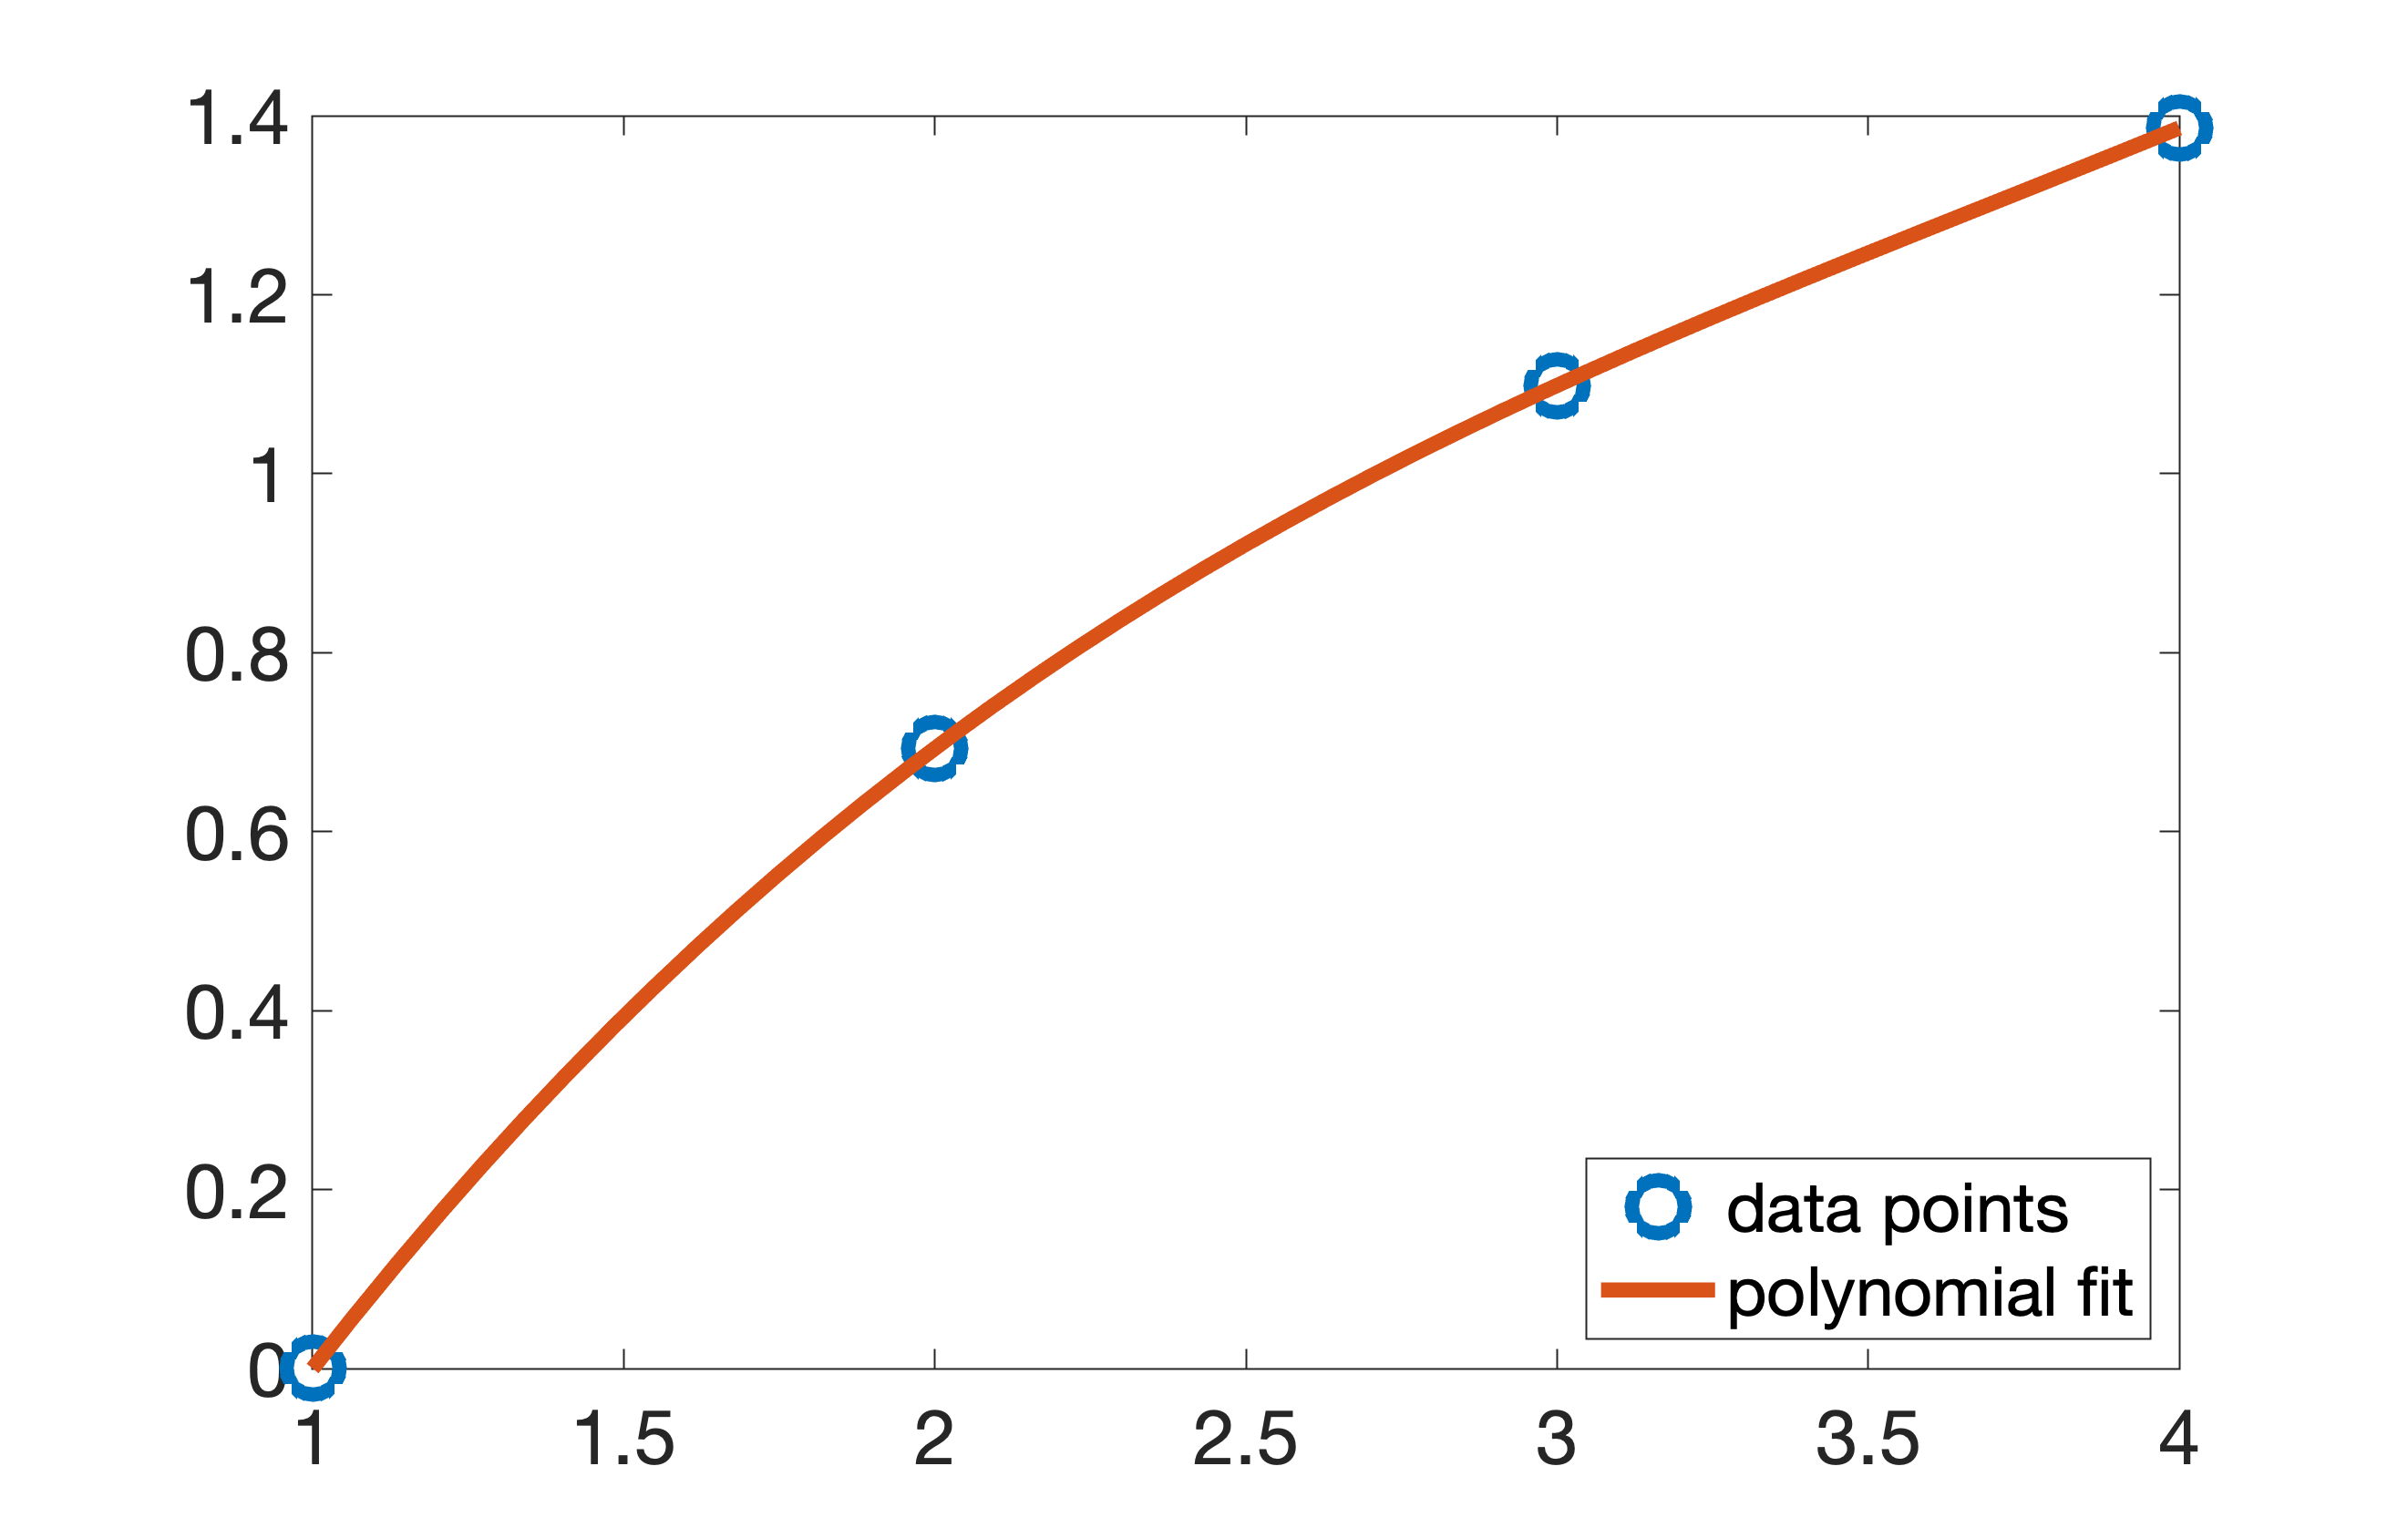
\includegraphics[width=0.7\linewidth]{./polyfit1.png}
\end{center}
}   

\begin{frame}[fragile]
\frametitle{Полиномы}
Если степень полинома, увеличенная на 1, меньше количества точек, то для определения коэффициентов полинома используется \alert{метод наименьших квадратов}:
\begin{lstlisting}
>> x = [ 1  2  3  4 ];
>> y = [ 0  0.6931  1.0986  1.3863 ];
>> p = polyfit(x, y, 2)

p =

    0.0283   -0.3137    1.4362   -1.1507
\end{lstlisting}
В этом случае полином не будет проходить через узловые точки ($x_i, y_i$)
\end{frame}

\frame[containsverbatim]
{
\frametitle{Построение графика}
\begin{center}
 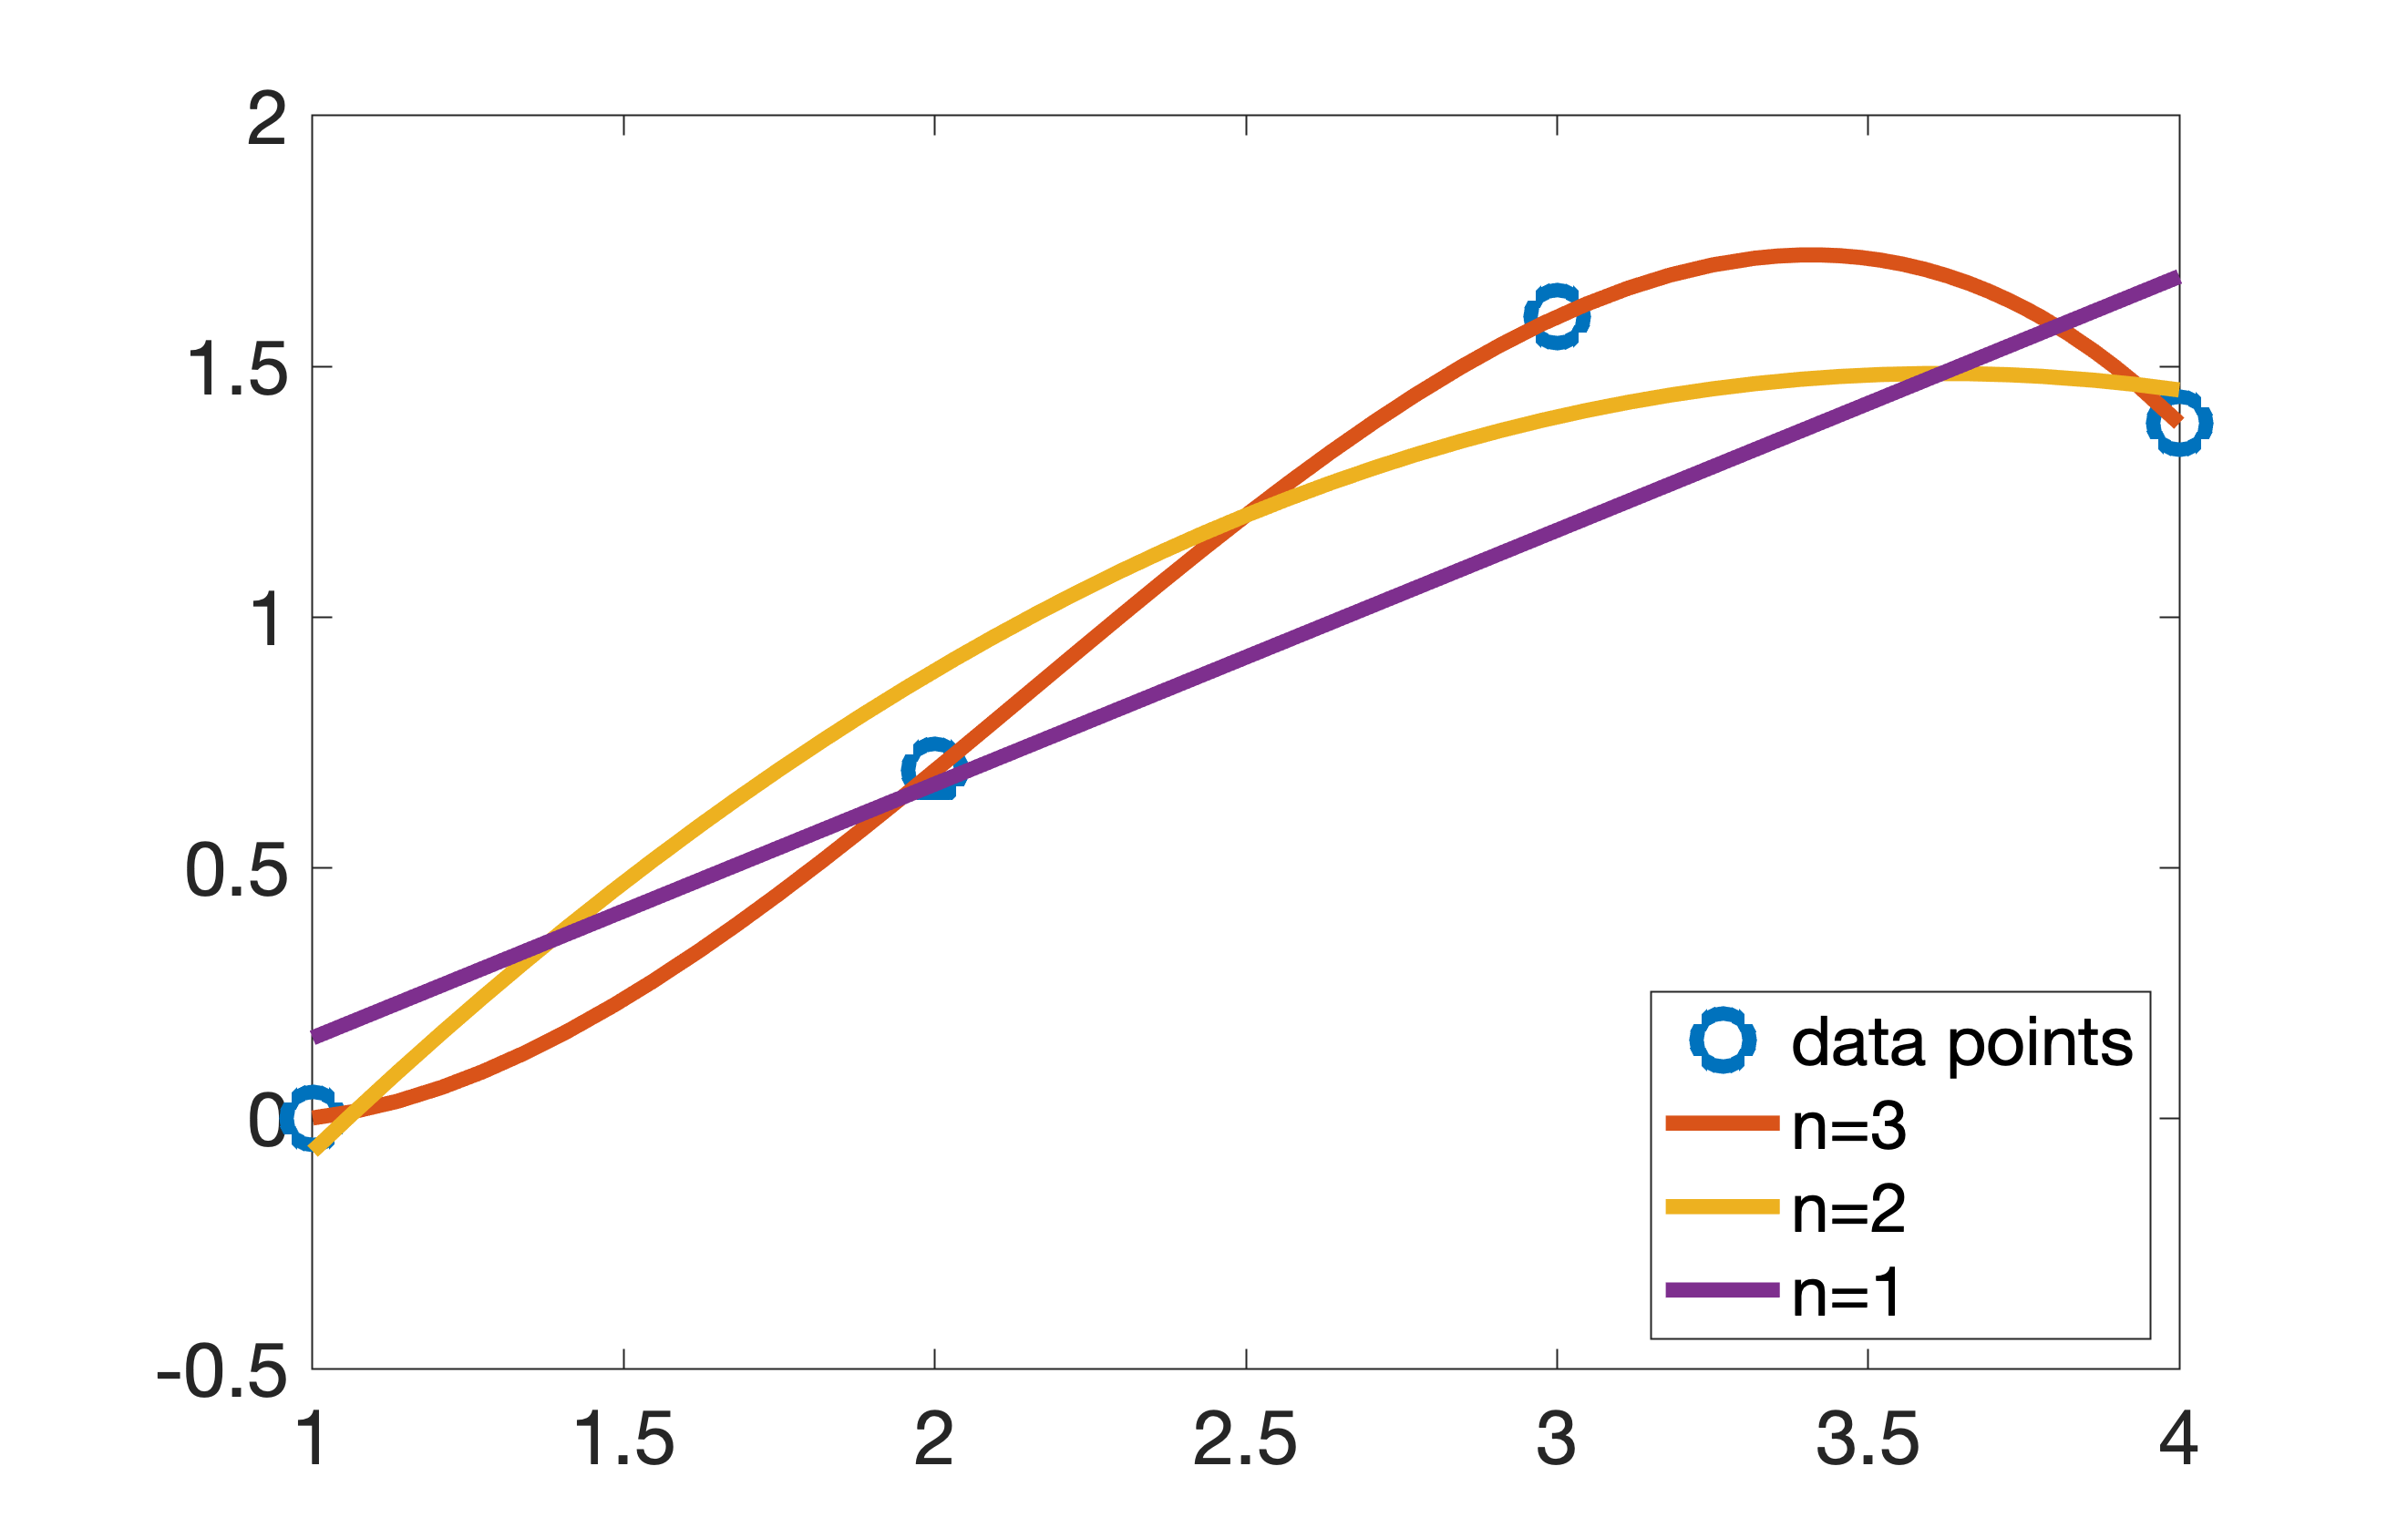
\includegraphics[width=0.8\linewidth]{./polyfit2.png}
\end{center}
}   


\frame[containsverbatim]
{
\frametitle{Полиномиальная интерполяция}
\begin{itemize}
 \item Полиномиальная интерполяция используется "локально". 
\begin{center}
 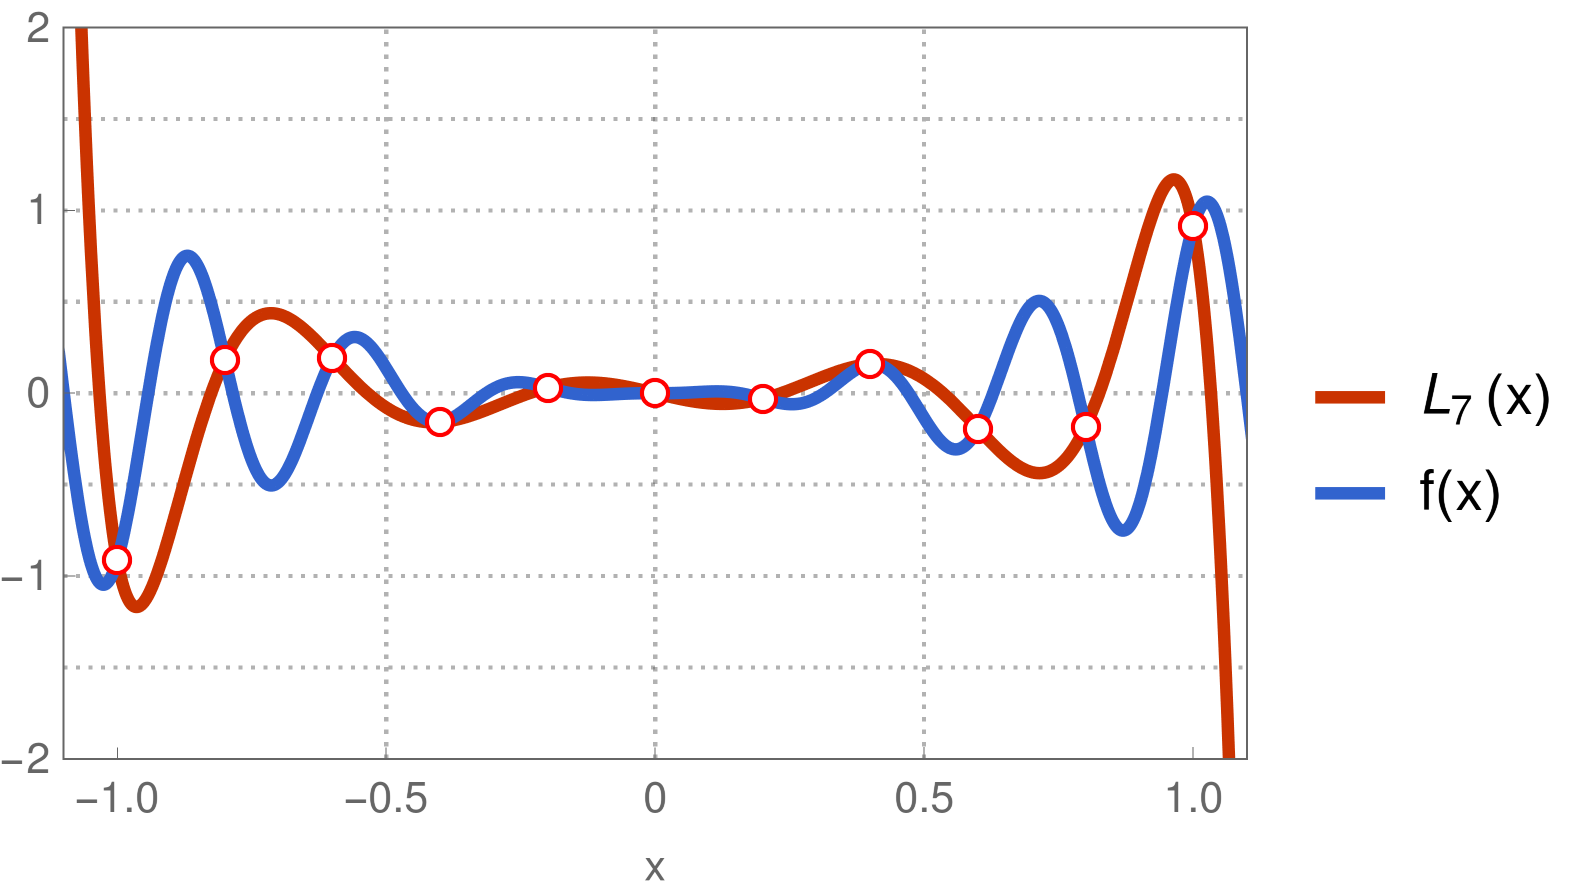
\includegraphics[width=0.7\linewidth]{./PolyInterpolationBad.png}
 % PolyInterpolation.png: 1573x847 pixel, 300dpi, 13.32x7.17 cm, bb=0 0 378 203
\end{center}
 \item Для глобальной интерполяции используется \emph{сплайн-интерполяция} -- глобальная "`кусочно-полиномиальная"' интерполяция. 
\end{itemize}
}

\begin{frame}[c,fragile]
\frametitle{Сплайн-интерполяция - interp1}    
\begin{lstlisting}        
interp1(x,y,xa,'linear');
\end{lstlisting}
Функция \emph{interp1} вычисляет значение табличной функции $y_i = f(x_i)$, заданной списком значений x и списком значений y, в точке xa, используя линейную интерполяцию. 
\end{frame}

\begin{frame}[t,fragile]
\frametitle{Сплайн-интерполяция - interp1}
\begin{lstlisting}
x = [ 1  2    3    4    5  ];
y = [ 0  0.6  1.0  1.7  1.1];

f = @(xa) interp1(x,y,xa,'linear');
\end{lstlisting}
\begin{center}
 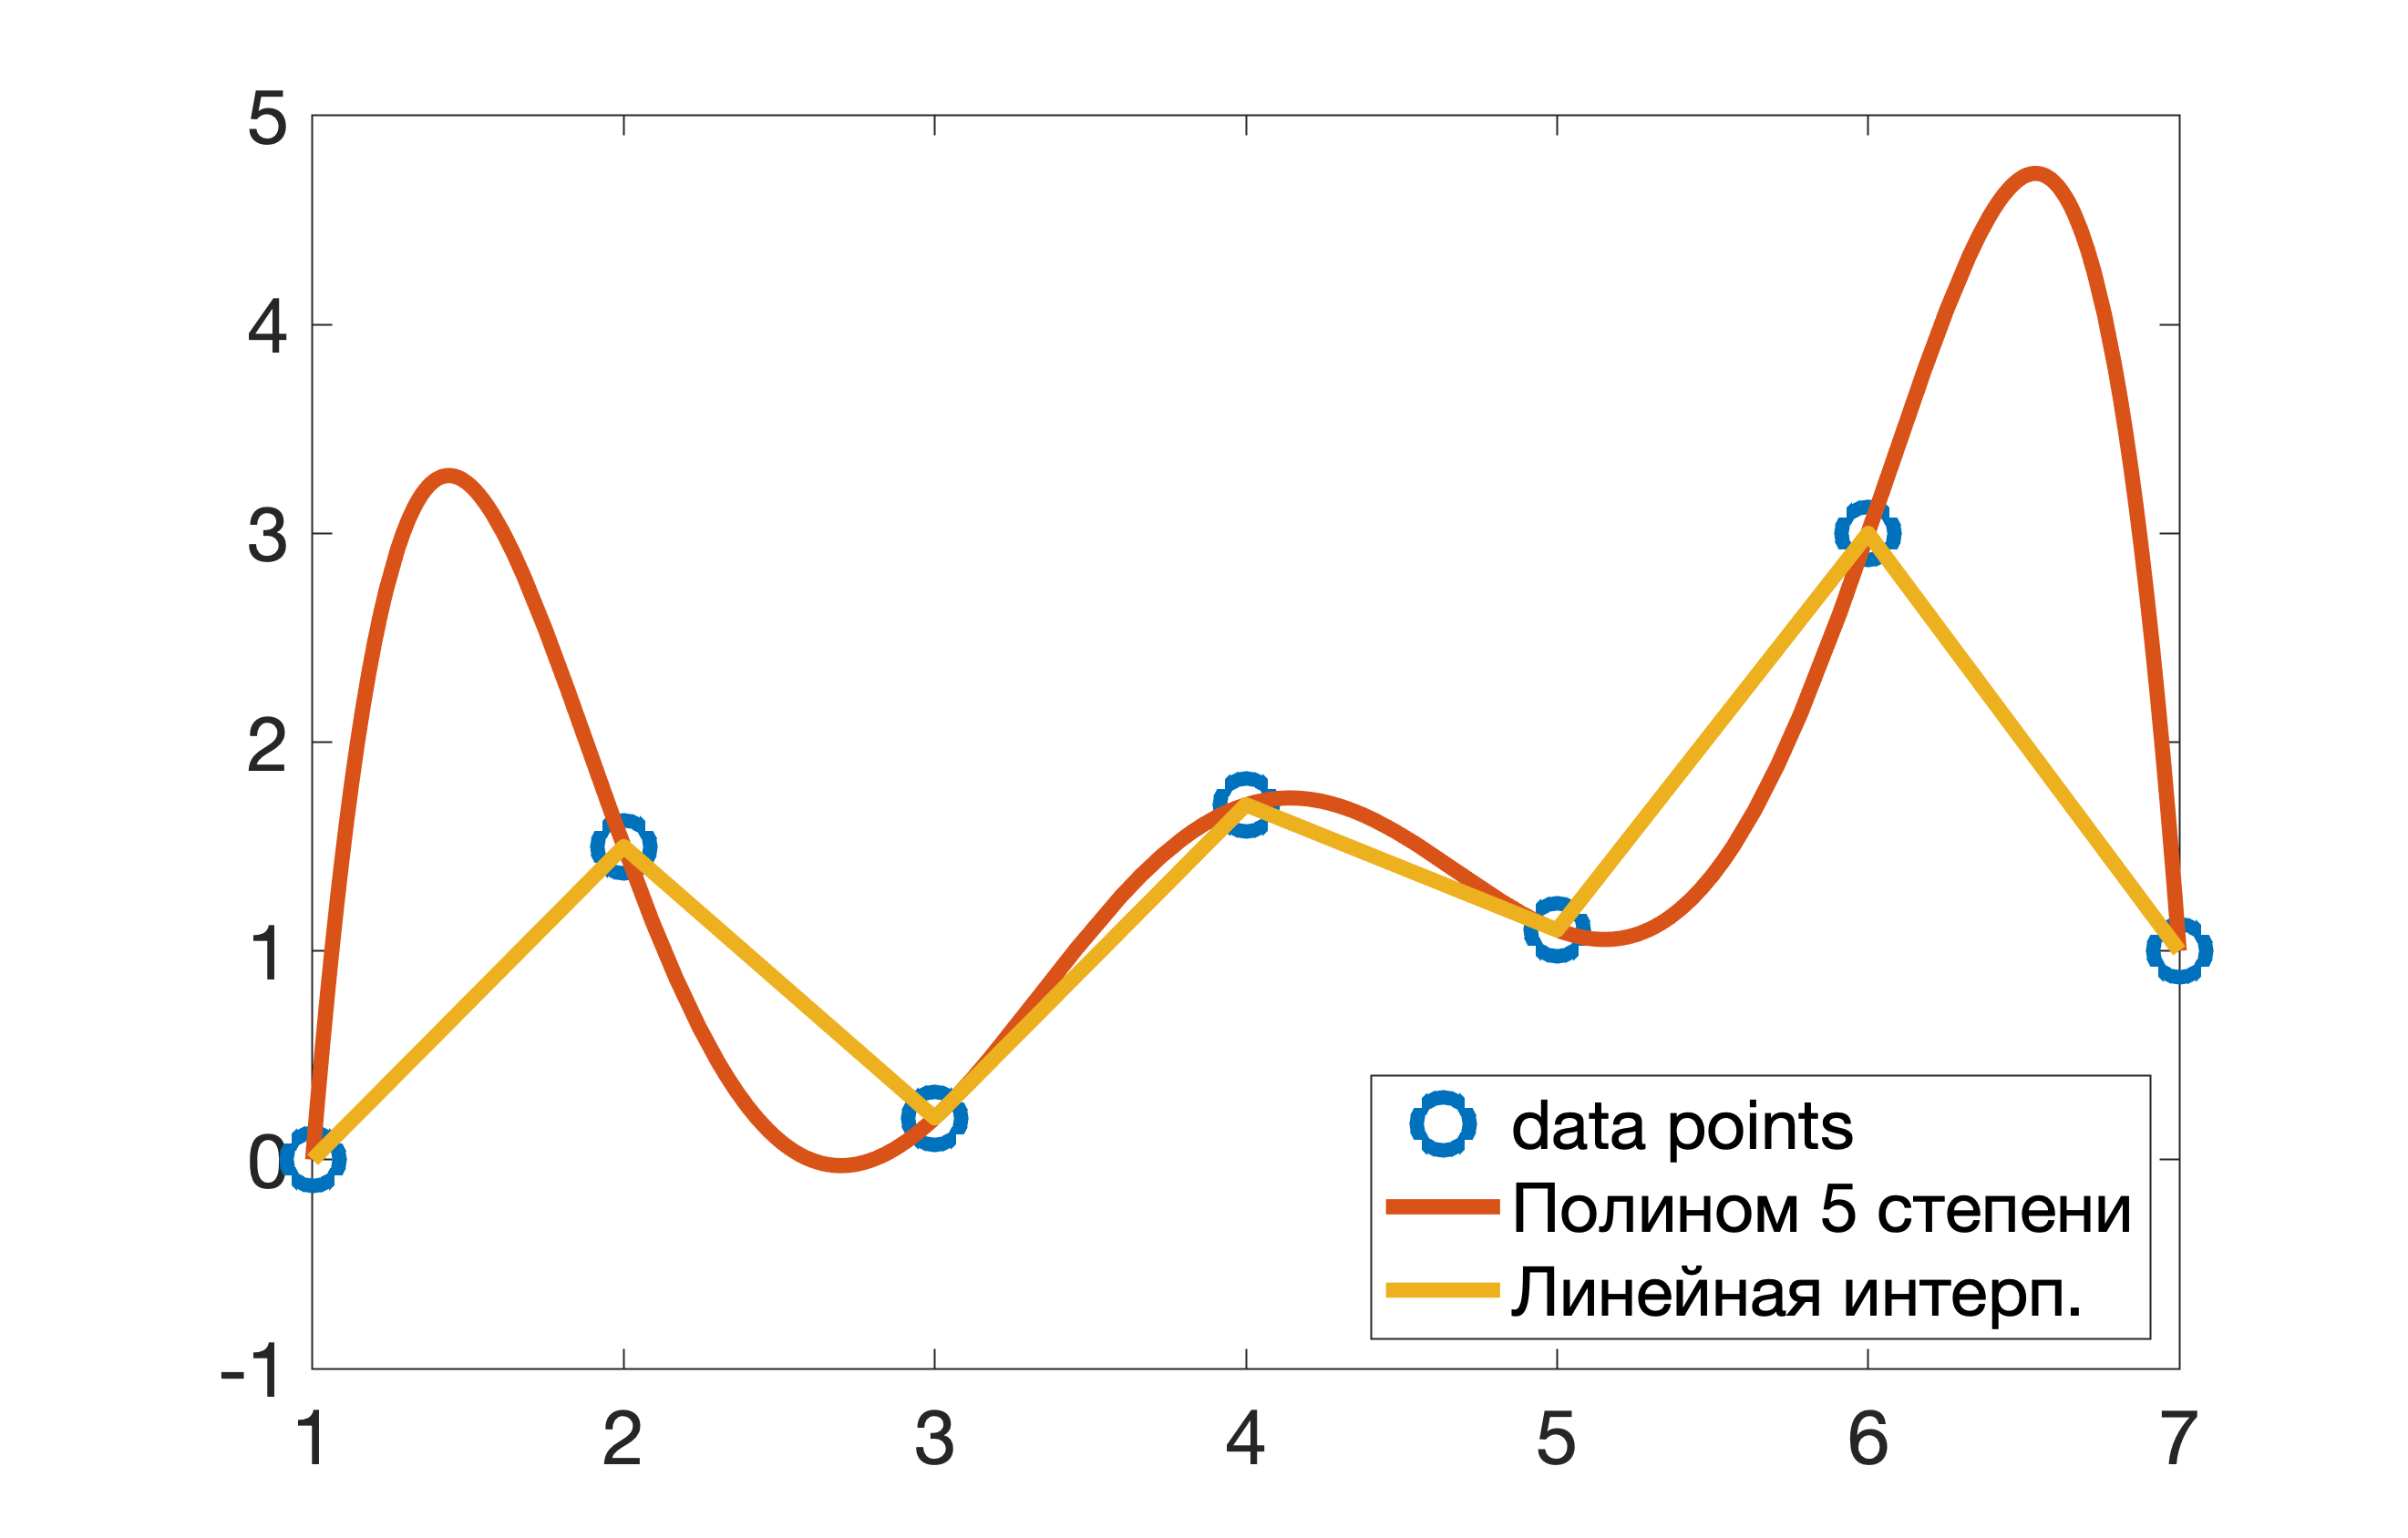
\includegraphics[width=0.7\linewidth]{./polyfit3.png}
\end{center}
\end{frame}

\begin{frame}[t,fragile]
\frametitle{Сплайн-интерполяция}
\begin{lstlisting}
x = [ 1  2    3    4    5  ];
y = [ 0  0.6  1.0  1.7  1.1];

f = @(xa) interp1(x,y,xa,'spline');
\end{lstlisting}
\begin{center}
 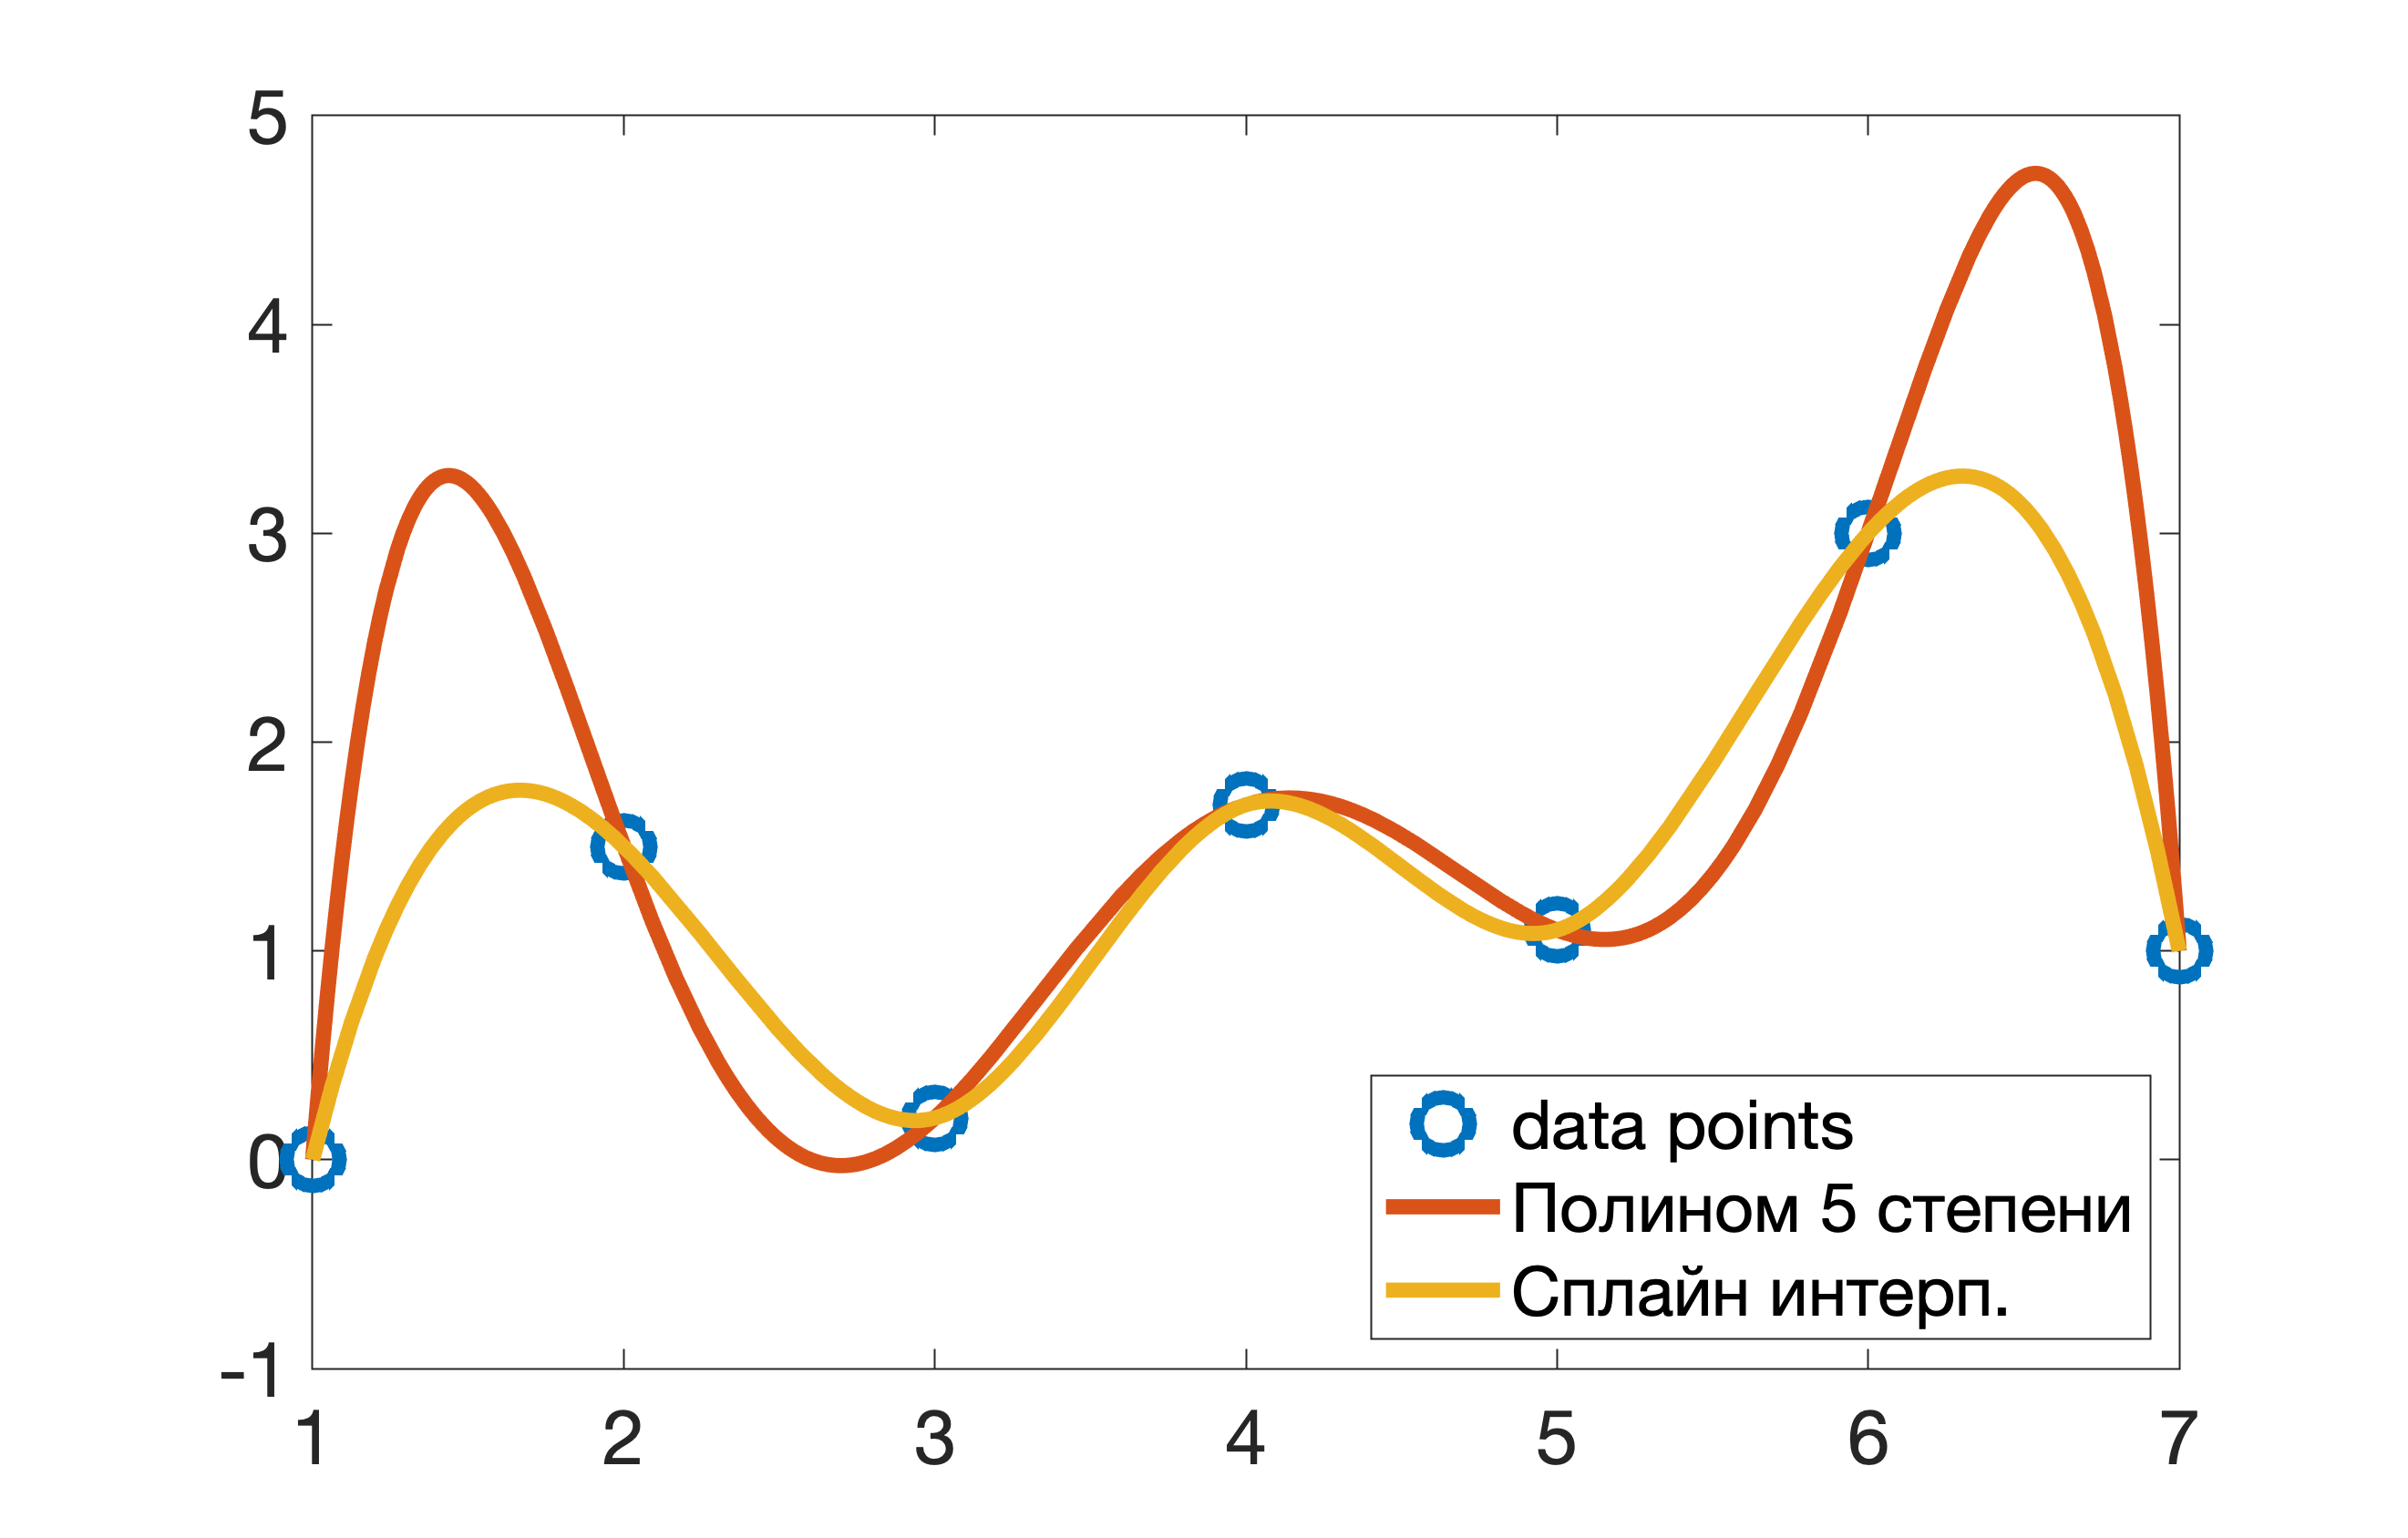
\includegraphics[width=0.7\linewidth]{./polyfit4.png}
\end{center}
\end{frame}

\section{Решение линейных уравнений}

\begin{frame}[t,fragile]
\frametitle{Системы линейных уравнений}
$$
\left\{
\begin{aligned}
    2 x_1 + 3 x_2 + x_3 = 5\\
    x_1 + 7 x_2 + 2 x_3 = 1\\
    3 x_1 + 2 x_2 + x_3 = 2
\end{aligned}
\right.
$$
\begin{lstlisting}
A = [2 3 1; 1 7 2; 3 2 1];
B = [5;1;2];

x = A\B

x =
    6.0000
    9.0000
  -34.0000
\end{lstlisting}
\end{frame}

\begin{frame}[t,fragile]
\frametitle{Системы линейных уравнений}
Решение двух систем, отличающихся столбцами правых частей, "в одно действие":
\begin{align*}
    2 x_1 + 3 x_2 + x_3 = 5 & \quad 2 x_1 + 3 x_2 + x_3 = 6 \\
    x_1 + 7 x_2 + 2 x_3 = 1 & \quad x_1 + 7 x_2 + 2 x_3 = 7 \\
    3 x_1 + 2 x_2 + x_3 = 2 & \quad 3 x_1 + 2 x_2 + x_3 = 1
\end{align*}
\begin{lstlisting}
A = [2 3 1; 1 7 2; 3 2 1];
B = [5 6; 1 7; 2 1];

x = A\B

x =
    6.0000    5.0000
    9.0000   10.0000
  -34.0000  -34.0000
\end{lstlisting}
\end{frame}

\section{Задачи линейного програмирования}

\begin{frame}[c]\frametitle{Линейное программирование}
Линейное программирование — это математический численный метод для оптимизации моделей, в которых целевые функции 
$$
    f(x_1,x_2,\ldots,x_n) \rightarrow min
$$
и ограничения, например
$$
    g(x_1,x_2,\ldots,x_n) > 0
$$
строго являются линейными уравнениями.
\end{frame}

\begin{frame}[c]\frametitle{Пример}

\begin{tabular}{c|c|c|c|c|c}
Вид сырья & Прод. 1 & Прод. 2 & Прод. 3 & Прод. 4 & Запас сырья \\
\hline
Сырье 1 & 4 & 2 & 1 & 8 & $\leq1200$ кг \\
Сырье 2 & 2 & 10 & 6 & 0 & $\leq600$ кг \\
Сырье 3 & 3 & 0 & 6 & 1 & $\leq1500$ кг \\
\hline
Прибыль & 15 р. & 6 р. & 12 р. & 24 р. & max \\
\end{tabular}
\vfill
Прибыль (целевая функция) $S = x_1 s_1 + x_2 s_2 + x_3 s_3 + x_4 s_4 \rightarrow max$

Ограничения
$$
	x_1 a_{11} + x_2 a_{12} + x_3 a_{13} + x_4 a_{14} \leq 1200
$$
$$
    x_1 a_{21} + x_2 a_{22} + x_3 a_{23} + x_4 a_{24} \leq 600
$$
$$
	x_1 a_{31} + x_2 a_{32} + x_3 a_{33} + x_4 a_{34} \leq 1500
$$
\end{frame}

\begin{frame}[c, fragile]\frametitle{Функция linprog}
\begin{lstlisting}
x = linprog(f,Ane,Bne,Ae,Be,lb,ub)
\end{lstlisting}
$$
\min_{x} \boldsymbol{f}^T x 
$$
При условиях равенствах
$$
	\boldsymbol{A}_e \boldsymbol{x} = \boldsymbol{B_e}
$$
При условиях неравенствах
$$
	\boldsymbol{A}_{ne} \boldsymbol{x} \leq \boldsymbol{B_{ne}}
$$
При условиии
$$
	\boldsymbol{L} \leq \boldsymbol{x} \leq \boldsymbol{U}
$$
\end{frame}

\begin{frame}[c,fragile]\frametitle{Пример}
\begin{tabular}{c|c|c|c|c|c}
Вид сырья & Прод. 1 & Прод. 2 & Прод. 3 & Прод. 4 & Запас сырья \\
\hline
Сырье 1 & 4 & 2 & 1 & 8 & $\leq1200$ кг \\
Сырье 2 & 2 & 10 & 6 & 0 & $\leq600$ кг \\
Сырье 3 & 3 & 0 & 6 & 1 & $\leq1500$ кг \\
Прибыль & 15 р. & 6 р. & 12 р. & 24 р. & max \\
\end{tabular}
\vspace{5mm}
\begin{lstlisting}
A = [4 2 1 8; 2 10 6 0; 3 0 6 1];
B = [1200; 600; 1500];
f = -[15 6 12 24];
x = linprog(f,A,B,[],[],[0 0 0 0],[])
\end{lstlisting}
x = [0 0 100 137.5]
\end{frame}

\section{Решение нелинейных уравнений}

\begin{frame}[fragile]
\frametitle{Функции одной переменной}
Для решения уравнений вида
$$
	f(x) = 0
$$    
используется функция \matcode{fzero}, первым аргументом которой является ссылка на функцию $f(x)$, вторым -- начальное приближение для искомого значения решения уравнения или интервал внутри которого находится решение:
\begin{lstlisting}
>> fzero( @(x) cos(x) - x, 1)

ans =

    0.7391
\end{lstlisting} 
\end{frame}

\begin{frame}[fragile]
\frametitle{Система нелинейных уравнений}
Для решения системы нелинейных уравнений используется функция \matcode{fsolve}. Например, для решения системы 
$$
	\left\{
	\begin{aligned}
	x^2 + y^2 + z^2 - 1 & = 0 \\ 
	2x^2 + y^2 - 4z  & = 0 \\ 
	3x^2 - 4y + z^2  & = 0 
	\end{aligned}
	\right.
$$
необходимо написать m-файл с векторной функцией векторного аргумента
\begin{lstlisting}
function y = f(x)
    y = [x(1)^2+x(2)^2+x(3)^2-1;
         2*x(1)^2+x(2)^2-4*x(3);
         3*x(1)^2-4*x(2)+x(3)^2];
\end{lstlisting}    
\end{frame}

\begin{frame}[fragile]
\frametitle{Система нелинейных уравнений}
Для поиска решения необходимо вызвать функцию \matcode{fsolve}, передав ей ссылку на функцию и вектор начального приближения $[x_0, y_0, z_0]$: 
\begin{lstlisting}
>> fsolve(@y,[1;1;1])

ans =

    0.7852
    0.4966
    0.3699
\end{lstlisting}
\end{frame}


\section{Поиск экстремума функции}

\begin{frame}[c,fragile]\frametitle{Функция fminbnd(fun,x1,x2)}
Поиск минимума фунции $f(x)$ на интервале $[x_1,x_2]$
\begin{lstlisting}
fun = @(x) x^2 - 0.3*x^3 + 3 + cos(4*x)^2;
fplot(fun,[-1 3]);
fminbnd(fun,-1,3)
ans = 
    0.372
\end{lstlisting}
\begin{center}
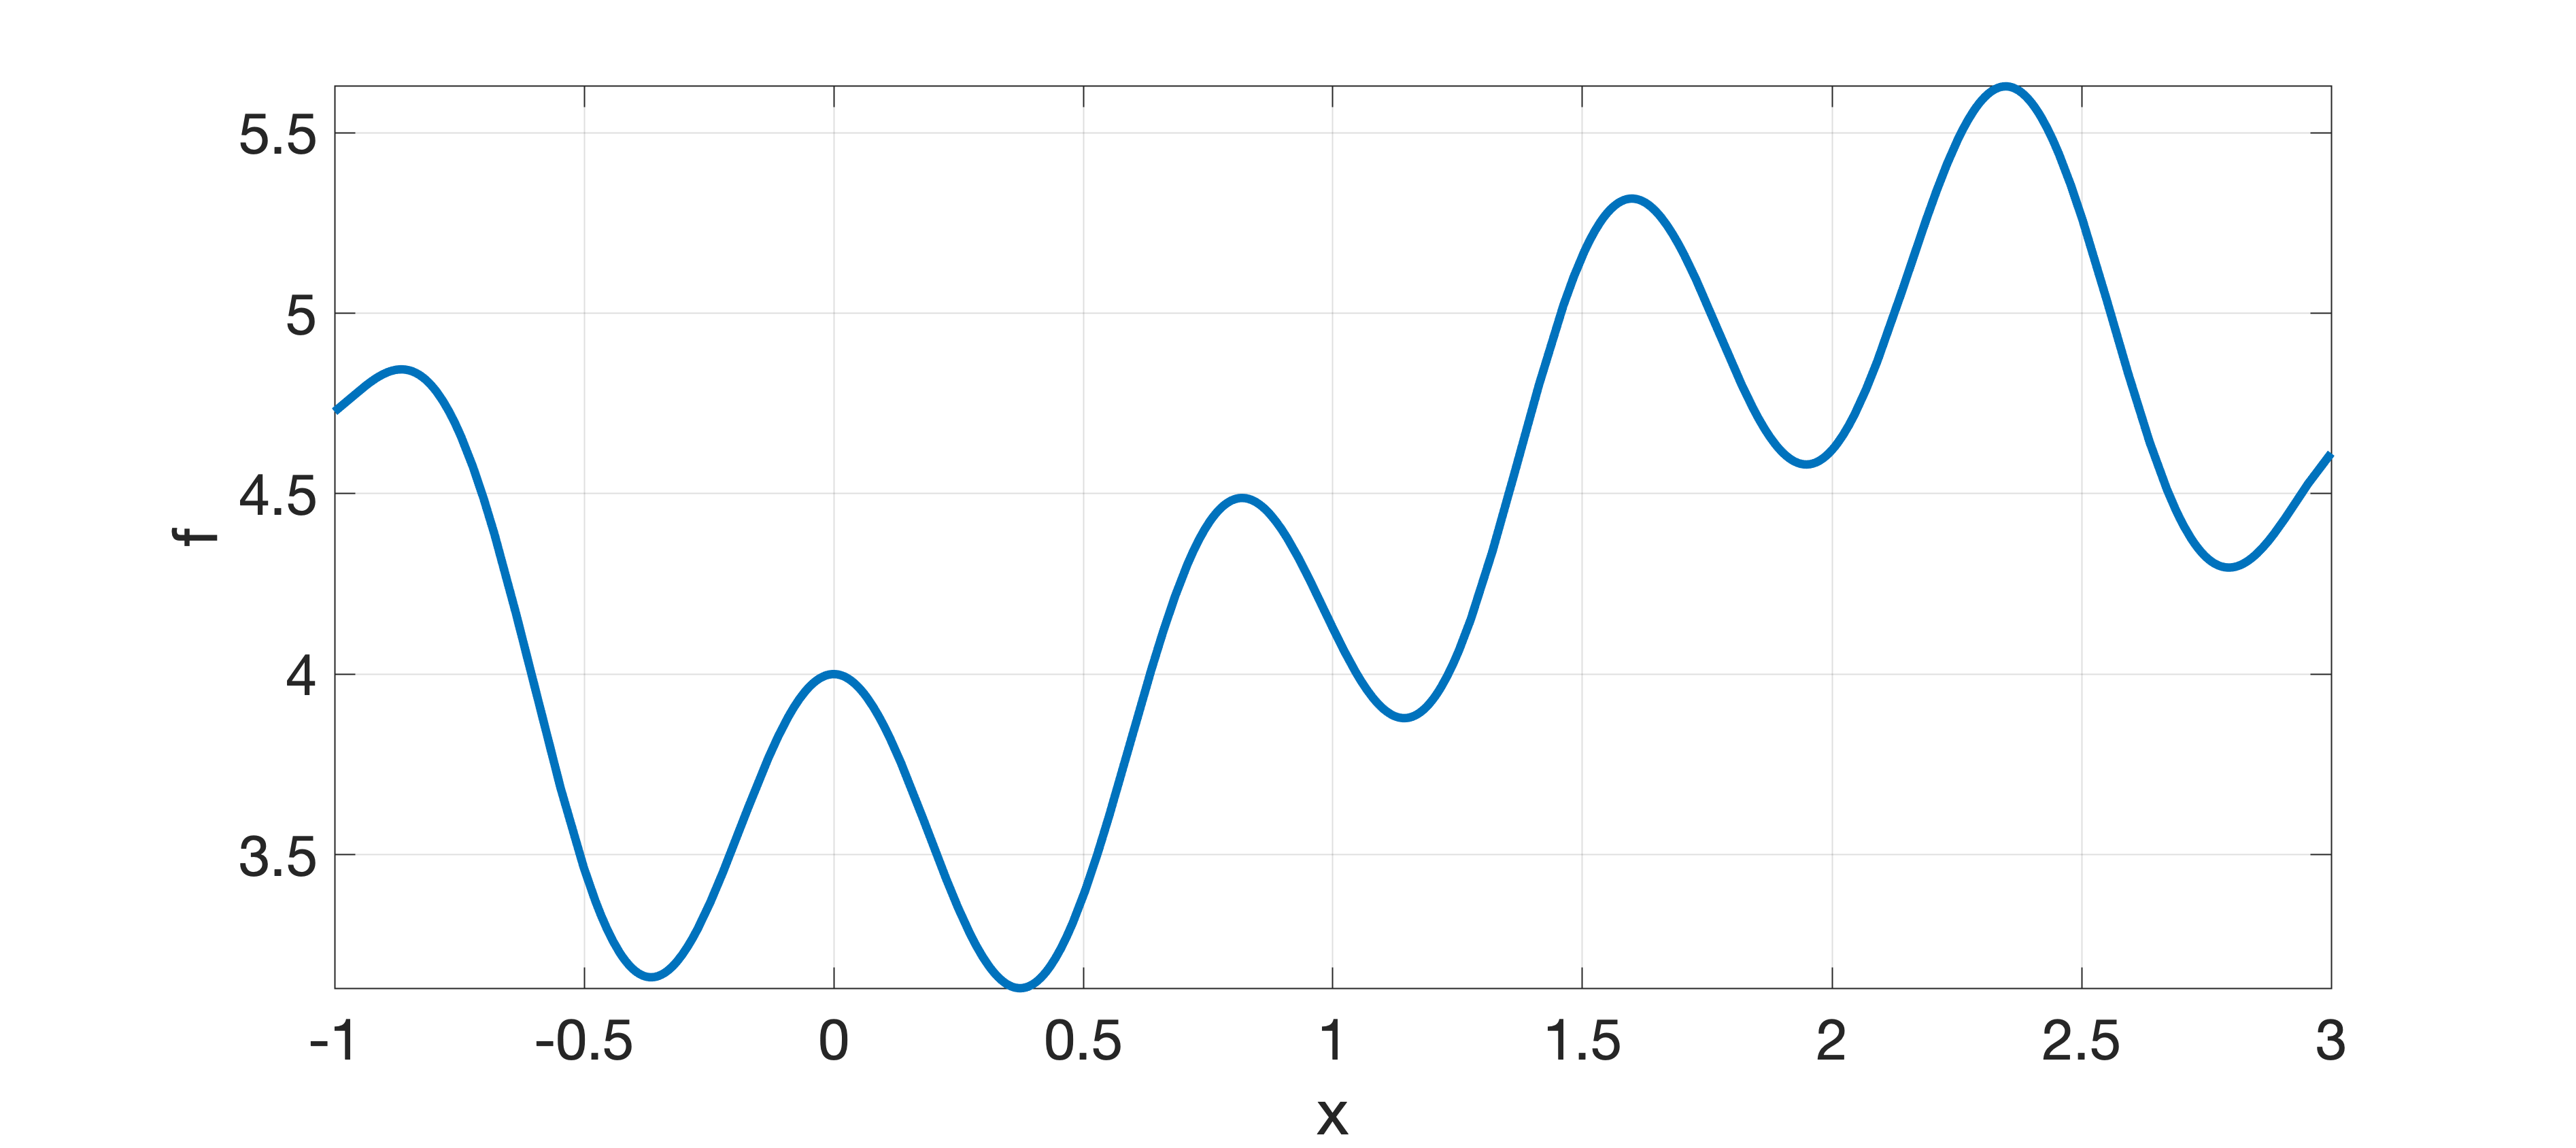
\includegraphics[width=0.8\textwidth]{fminbnd.png}
\end{center}
\end{frame} 

\begin{frame}[c,fragile]
\frametitle{Функция нескольких переменных}
Найти минимум функции нескольких переменных
$$
    \min_{\boldsymbol x} f(\boldsymbol x), \quad \boldsymbol{x} = [x_1,x_2,\ldots,x_n]
$$
Пример:
$$ 
f(x)=100(x_2 − x_1^2)^2+(1−x_1)^2
$$
\begin{lstlisting}
fun = @(x1,x2) 100*(x2-x1.^2).^2+(1-x1).^2;
\end{lstlisting}
\end{frame} 

\begin{frame}[c,fragile]
\frametitle{Функция нескольких переменных}
\begin{lstlisting}
x1 = linspace(0,3,100);
x2 = linspace(0,3,100);
[X1,X2] = meshgrid(x1,x2);
f = fun(X1,X2);
contour(X1,X2,f,200);
\end{lstlisting}
\begin{center}
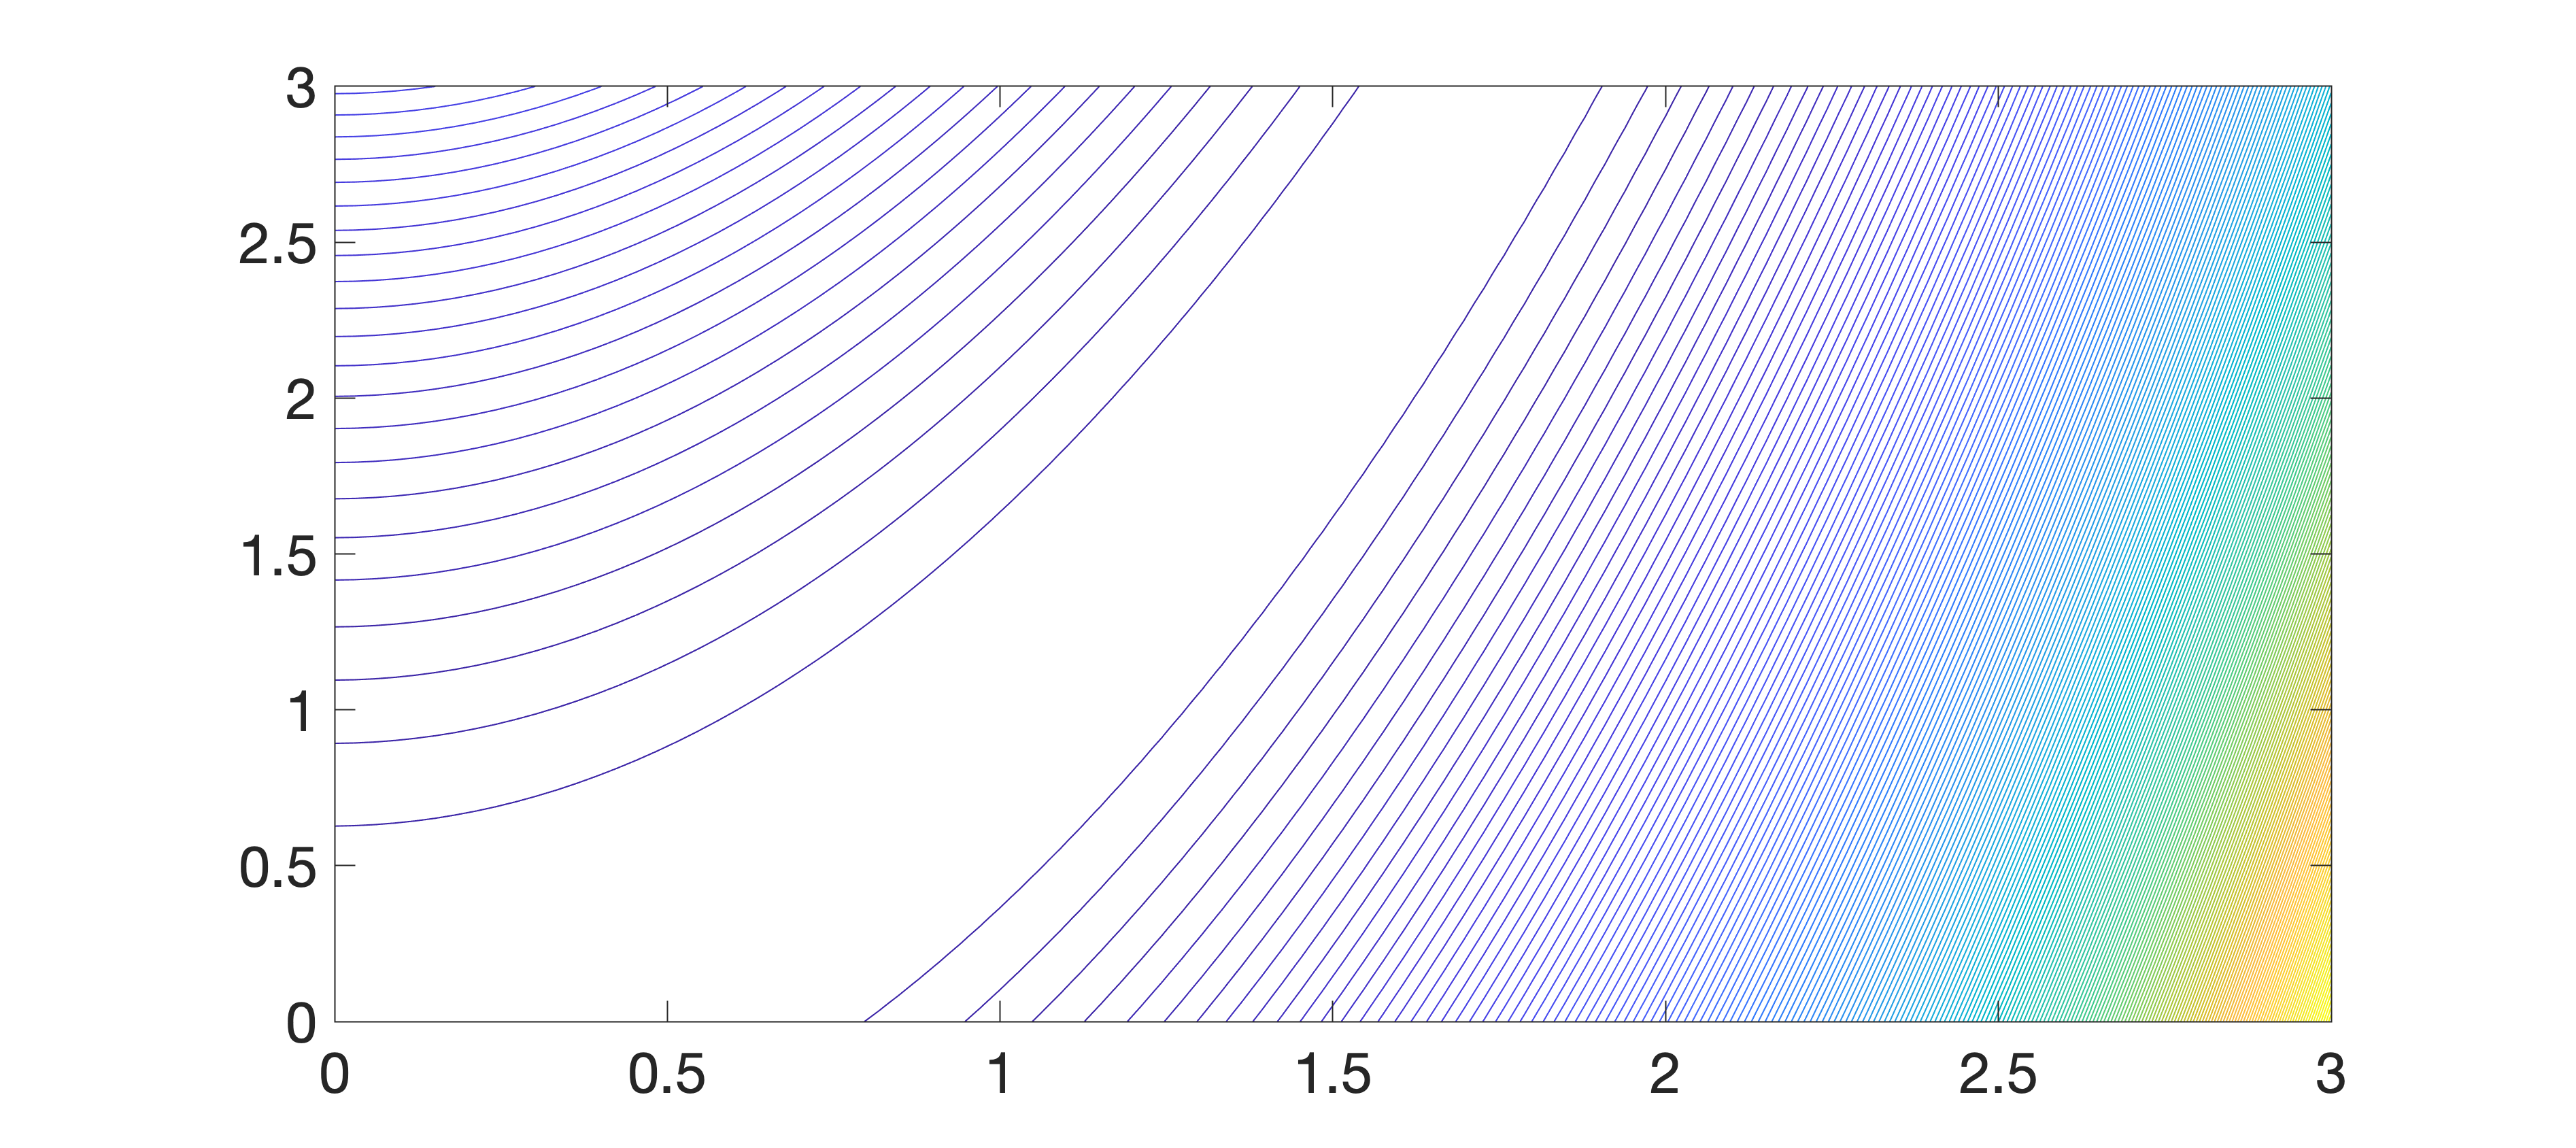
\includegraphics[width=0.8\textwidth]{fminsearch.png}
\end{center}
\end{frame} 

\begin{frame}[c,fragile]
\frametitle{Функция fminsearch}
Функция \emph{fminsearch}
\begin{lstlisting}
fminsearch(@(x) fun(x(1),x(2)),[0, 0.5])

ans =

    1.0000    1.0000
\end{lstlisting}
Аргументы функции fminsearch
\begin{itemize}
    \item ссылка на функцию от \emph{векторного аргумента}
    \item начальное приближение
\end{itemize}
\end{frame} 


\section{Численное дифференцирование}

\begin{frame}[t,fragile]
\frametitle{Функция diff}
Разность первого порядка
$$
	\Delta y_i = y_{i+1} - y_{i}
$$
\begin{lstlisting}
x1 = 1; xn = 2; h=0.1;
x = x1:h:xn;
y = log(x);
dy = diff(y)

 0         0.0953    0.1823    0.2624    0.3365 ...
 0.0953    0.0870    0.0800    0.0741    0.0690 ...
\end{lstlisting}
\end{frame}

\begin{frame}[t,fragile]
\frametitle{Функция diff}
Разность второго порядка
$$
	\Delta^2 y_i = \Delta y_{i+1} - \Delta y_{i}
$$
\begin{lstlisting}
d2y = diff(y,2)

-0.0083   -0.0070   -0.0059   -0.0051   ...
\end{lstlisting}
\end{frame}

\begin{frame}[t,fragile]
\frametitle{Производная первого порядка}
Для внутренних узлов
$$
	y'(x_i) = \frac{\Delta y_{i-1} - \Delta y_{i}}{2h} = \frac{y_{i+1} - y_{i-1}}{2h}
$$
\begin{lstlisting}
dy  = diff(y);

dfi = @(i) (dy(i-1)+dy(i))/(2*h);

[x(2) dfi(2)]

ans =

    1.3000    0.7708
\end{lstlisting}
Точное значение 0.7692 (0.2\%)
\end{frame}

\begin{frame}[c]
\frametitle{Производная первого порядка}
Для внешнего узла $i=1$
$$
    y'(x_1) = \frac{\Delta y_{1} - \Delta^2 y_{1}/2}{2h}
$$
Для внешнего узла $i=n$
$$
    y'(x_n) = \frac{\Delta y_{n-1} - \Delta^2 y_{n-2}/2}{2h}
$$
\end{frame}

\begin{frame}[c,fragile]
\frametitle{Вторая производная}
$$
  y''(x_i) = \frac{\Delta y_i - \Delta y_{i-1}}{h^2}  
$$
\begin{lstlisting}
x    = x1:dx:x2;    
y    = some_math_function(x);
dy   = diff(y);        
dydt = @(i) (dy(i) - dy(i-1))/dx^2;
\end{lstlisting}
\end{frame}

\begin{frame}[t,fragile]\frametitle{Пример}
\small
\begin{lstlisting}
dx = 0.05;      
x  = (0:dx:0.5)';
y  = sin(x); yp = cos(x); ypp =-sin(x);

dy  = diff(y);
d2y = diff(y,2);

ypa  = @(i) (dy(i-1) + dy(i))/(2*dx);
yppa = @(i) (dy(i) - dy(i-1))/dx^2;

ind  = 2:numel(x)-1;
res  = [x(ind) yp(ind) ypa(ind) ypp(ind) yppa(ind)]

    0.1000    0.9950    0.9946   -0.0998   -0.0998
    0.2000    0.9801    0.9797   -0.1987   -0.1986
    0.3000    0.9553    0.9549   -0.2955   -0.2955
    0.4000    0.9211    0.9207   -0.3894   -0.3893
\end{lstlisting}
\end{frame}

\section{Численное интегрирование}

\begin{frame}[fragile]
\frametitle{Формула трапеций}
Для функции, заданной таблично, интеграл можно вычислить используя формулу трапеций: 
\begin{lstlisting}
>> x = 1.0:0.1:2.0;
>> y = log(x);

>> trapz(x, y)

ans =

    0.3859
\end{lstlisting}    
Точное значение интеграла равно $\log 4 - 1 \approx 0.386294361119891$.
\end{frame}

\begin{frame}[fragile,c]
\frametitle{Функция quad (intergral)}
Для известной подинтегральной функции более точный результат дает использование функции \matcode{quad}, в которую нужно передать ссылку на подинтегральную функцию и пределы интегрирования
$$
\int_1^2 \ln(x) dx 
$$
\begin{lstlisting}
>> format long
>> quad(@log, 1, 2)

ans =

   0.386294334336416
\end{lstlisting}
\end{frame}

\begin{frame}[fragile,c]
\frametitle{Функци quad (intergral)}
Третьим аргументом функции \matcode{quad} является желаемая точность результата (по умолчанию -- $10^{-6}$)
\begin{lstlisting}
f = @(x) sin(x).*log(x).^2;

quad(f, 1, 2, 1e-8)

ans =
   0.1822
\end{lstlisting}
Функция \matcode{integral} 
\begin{lstlisting}
integral(f, 1, 2, 'AbsTol', 1e-8)   

ans =
   0.1822
\end{lstlisting}
\end{frame}


\end{document}
